\chapter{Results}
\label{results}

\section{Measurement and validation}

\subsection{Ea}  % Integration of Force/Disp curves
\label{sec:Ea}

As previously stated, one of the main purpouses of the studied devices is to absorb the biggest amount of energy on an impact.

The total amount of dissipated energy, by whichever mechanisms, will be equal to the total input energy. Therefore, \gls{Ea} would, ideally, be the result of integrating the displacement multiplied by the force during the defformation, as indicated in equation \ref{eq:Ea_concept}.

\begin{equation}
E_a = \int_{s_0}^{s_f} F(s) \mathrm{d}s
\label{eq:Ea_concept}
\end{equation}
% \caption{Concept of energy absorption}

where $s$ is the displacement; $s_0$ and $s_f$ are the initial and final displacements; and $F(s)$ is the force for that differential increment of displacement. Equation \ref{eq:Ea} is an adaptation of equation \ref{eq:Ea_concept} that is used in this study.

\begin{equation}
E_a \approx \displaystyle\sum_{i=0}^{N-1} \frac{F_{i+1}^R+F_{i}^R}{2} \left(s_{i+1}-s_{i}\right)
\label{eq:Ea}
\end{equation}
% \caption{Energy absorption calculation method}

where $N$ is the total amount of output steps. The superindex $R$ affecting the force term stands for ``rear'', as its measured in the rear plate in order to prevent too much noise in the output.

\Gls{SEA} can be obtained by dividing \gls{Ea} by the total mass of the specimen \citep{Lee2006, Peroni2009, Scattina2011}. This output parameter is also used to validate the model, toghether with \ref{sec:F-D}, by comparing the obtained values with those obtained by \citet{Peroni2009}. Although some differences may appear, their origin is in the discrepancies on \ref{sec:F-D}.

\subsection{F-D}
\label{sec:F-D}

Typical crash test \glspl{F-D} present a series of alternating peaks and valleys of similar values, except for the first peak, which is greater in value (about twice or three times the mean value) and much more pronounced. Except in case of \ref{sec:critical_sits}, \gls{Pk} takes place in this first peak.

\begin{figure}
\centering
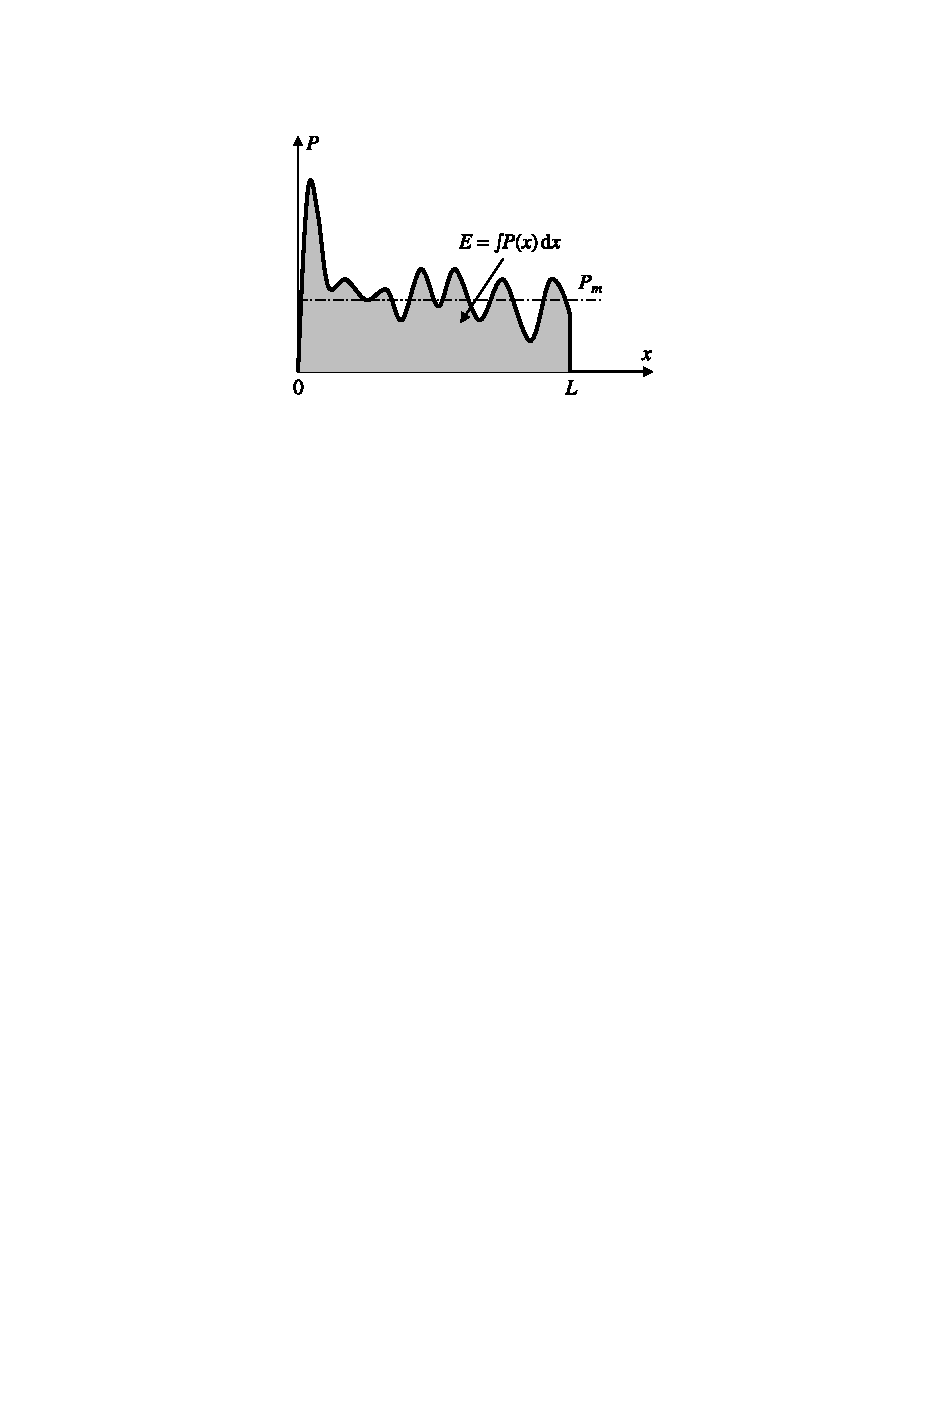
\includegraphics[angle=0,width=0.8\columnwidth]{f-d}
\caption{Typical force-displacement curve in a crash test. Taken from \citep{Scattina2011}}
\label{fig:damage_evo2D}
\end{figure}

Obtained curves present a first peak of $\SI{60~65}{\kN}$ in the beginning of the impact, and then a series of peaks, less pronounced and lower in value, alternating with valleys during the wave formation \ref{sec:wave_formation}, with a mean value of $\SI{20~25}{\kN}$.

% Insert obtained F-D curve

\begin{figure}
\centering
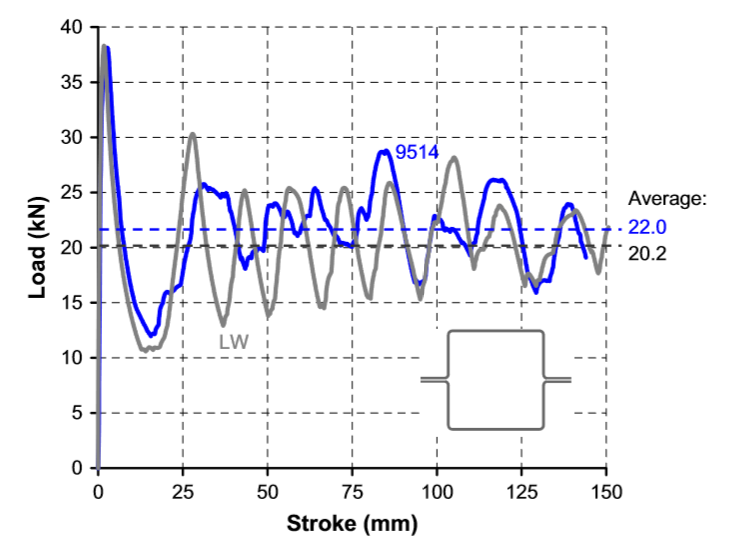
\includegraphics[angle=0,width=0.8\columnwidth]{peroni_qstat_fd}
\caption{Force-displacement curve obtained in quasi-static test for studied adhesive and other bonding solution. Taken from \citep{Peroni2009}}
\label{fig:damage_evo2D}
\end{figure}

Qualitativelly, this curves are very similar to those obtained by \citet{Peroni2009}; facing these similitudes, the model is considered valid.

The main exception to these similitudes can be found on the first peak, which progressivelly reduces its value after happening, instead of rapidly dropping its magnitude to the peaks and valleys series' mean. Because of this, the last peak does not take place within the studied interval.

\section{Collapse mechanism}

The origin of mentioned difference may be related to the collapse mechanism. Specifically, to the rate of changing the response mechanism for the crash box, from in-plane compression of the plates ---which is directly related to the \gls{Pk}---, to the initiation of \ref{sec:wave_formation}. In the developped model, if compared to the collapse images provided by \citet{Scattina2011}, this rate is far slower.

\subsection{Wave formation}
\label{sec:wave_formation}
Apart from happening on the impact head, wave formation may take also place in the opposite end of the tube or in some mid-point \citep{Abedrabbo2009, Costas2013} in this slender crash devices.

\subsection{Critical situations}
\label{sec:critical_sits}
\citet{Peroni2009} found several situations in impact tests in which the expected collapse mechanism wasn't achieved. Instead, bonding rapidly failed, making only use of the plate's capabilities to absorb the impact through its elasto-plastic defformation like bending shells without wave formation.

When this situation takes place, \gls{Ea} gets drastically reduced. During the study development, it was found that this critical situations can drop \gls{SEA} to a half or even a third of the expected values if compared with non-critical values given by \citet{Peroni2009}.

This section aims to expose some of the most common critical situations found during the study development, usually by changing the boundary conditions affecting the tube. The reasons involved in this malfunctioning are related and always present combined.

\subsubsection{Triggering missfunctions}  % Head aperture
\label{sec:trig_missf}

\subsubsection{General bending}

It was found that in many cases, during \ref{sec:wave_formation}, a minor difference between plates defformation, eventually resulted in the box bending by some mid-point, diverting the tube's directrix instead of crushing the device in a straight direction.

% Insert image

Analyzing the origin of this situation, several possible reasons were considered:
\begin{itemize}
\item A longer wave on one side, followed by a less pronounced one. Membrane effect on the former one makes it a stiffer point. The last one is a weak section, as the consecutive adherend planes are folding toghether. As this situation only takes place on one of the adherends, the faux-symmetry ceases to exist, thus bending the tube by some mid-point.
\item Following a behaviour similar to that one found in \ref{sec:trig_missf}, aperture of the section happens in some mid-point. Usually an excesivelly opened wave by the union plane, sided by two under-formated waves that cannot compensate the aperture, triggers this failure.
\end{itemize}
% Insert images if possible

\subsubsection{General peeling due to plates buckling}

Excesivelly thick adherend plates prevent wave formation, resulting in other collapse mechanisms' development, such as a buckling-like defformation, as a beam subjected to high compression. In this situation, each plate bends to a side, peeling the union in the process.

% Insert image & maybe comment

\section{Interpretation}  % Include different geoms comparation if possible

\section{Conclusions}

The following conclusions can be deduced from the study results:
\begin{itemize}
\item Critical situations suppose an important type of response of the crash box.
\end{itemize}